The evaluation of our prototype consists of two parts: path discovery and bug finding. In path discovery, we evaluated different seed search method on several real world binary programs, and in bug finding, a demo program which contains several bugs, as well as another benchmark based on real world program, are leveraged to demonstrate the ability of our prototype system on bug finding.

\subsection{Path Discovery}
To evaluate the path discovery ability of our directed seed search method, we selected 8 programs which cover different input formats like executables, images, archives and network data. This evaluation was tested with one AFL node and lasted for 24 hours. The evaluation results were shown in Table~\ref{PD-8samples}. We have tested for four different kinds of search method, i.e. Orderly, Euclidean Distance, Cosine Similarity and Jaccard Index. The orderly search method is equal to vanilla AFL which selects test case in the seed queue one by one.  

\begin{table}
  \caption{\label{PD-8samples}Path discovery for 8 sample programs}
  \centering
	\begin{tabular}{p{2cm}<{\centering} p{1.5cm}<{\centering} p{1.5cm}<{\centering} p{1.5cm}<{\centering} p{1.5cm}<{\centering}}
		\toprule
		Program  & Order\# & EU\# & CS\# & JI\# \\ 
		\midrule
		readelf  &    2753 & 4595 & 5314 & 5062 \\
		 djpeg   &    2802 & 3020 & 4198 & 3390 \\
		objdump  &    1755 & 2200 & 2960 & 2133 \\
		  gzip   &    1440 & 1564 & 1754 & 1588 \\
		 ffmpeg  &    5022 & 5993 & 6181 & 5801 \\
		tcpdump  &    3399 & 3673 & 4267 & 2950 \\
		capstone &    5626 & 6008 & 6066 & 5873 \\
		gif2png  &     912 &  981 & 1100 &  997 \\ 
		\bottomrule
	\end{tabular}
\end{table}

Figure~\ref{path-discovery} shows the normalized path discovery for these 8 programs. From this figure, we can see that CS can achieve higher path coverage when comparing with other search strategies. And EU can also cover more paths than vanilla AFL but the performance is lower than CS. Compared with the other two distance measures, JI is the most unstable strategy which shows high path coverage for some benchmarks, like \texttt{readelf}, \texttt{djpeg}, but also brings performance loss for some other benchmarks, like \texttt{tcpdump}. 

Figure~\ref{path-detail} describes these four different search strategies for four different samples according to the test time, where the x-axis of each graph indicates the test time in hours; while the y-axis shows the normalized path discovery of each strategy.

From Figure~\ref{path-detail}, both CS and EU performed consistently better than orderly during all the 24 hours. Particularly, EU performed better than CS in the first several hours, and then CS outperformed EU in the following testing. While JI performed well in \texttt{readelf}, \texttt{ffmpeg} and \texttt{objdump}, but it failed to improve the performance in \texttt{tcpdump} after testing for 8 hours.

Based on this result, we can see that cosine similarity based seed search strategy can touch more paths than other strategies. So we selected CS as our search strategy in the following bug finding evaluation.

\begin{figure}
\centering
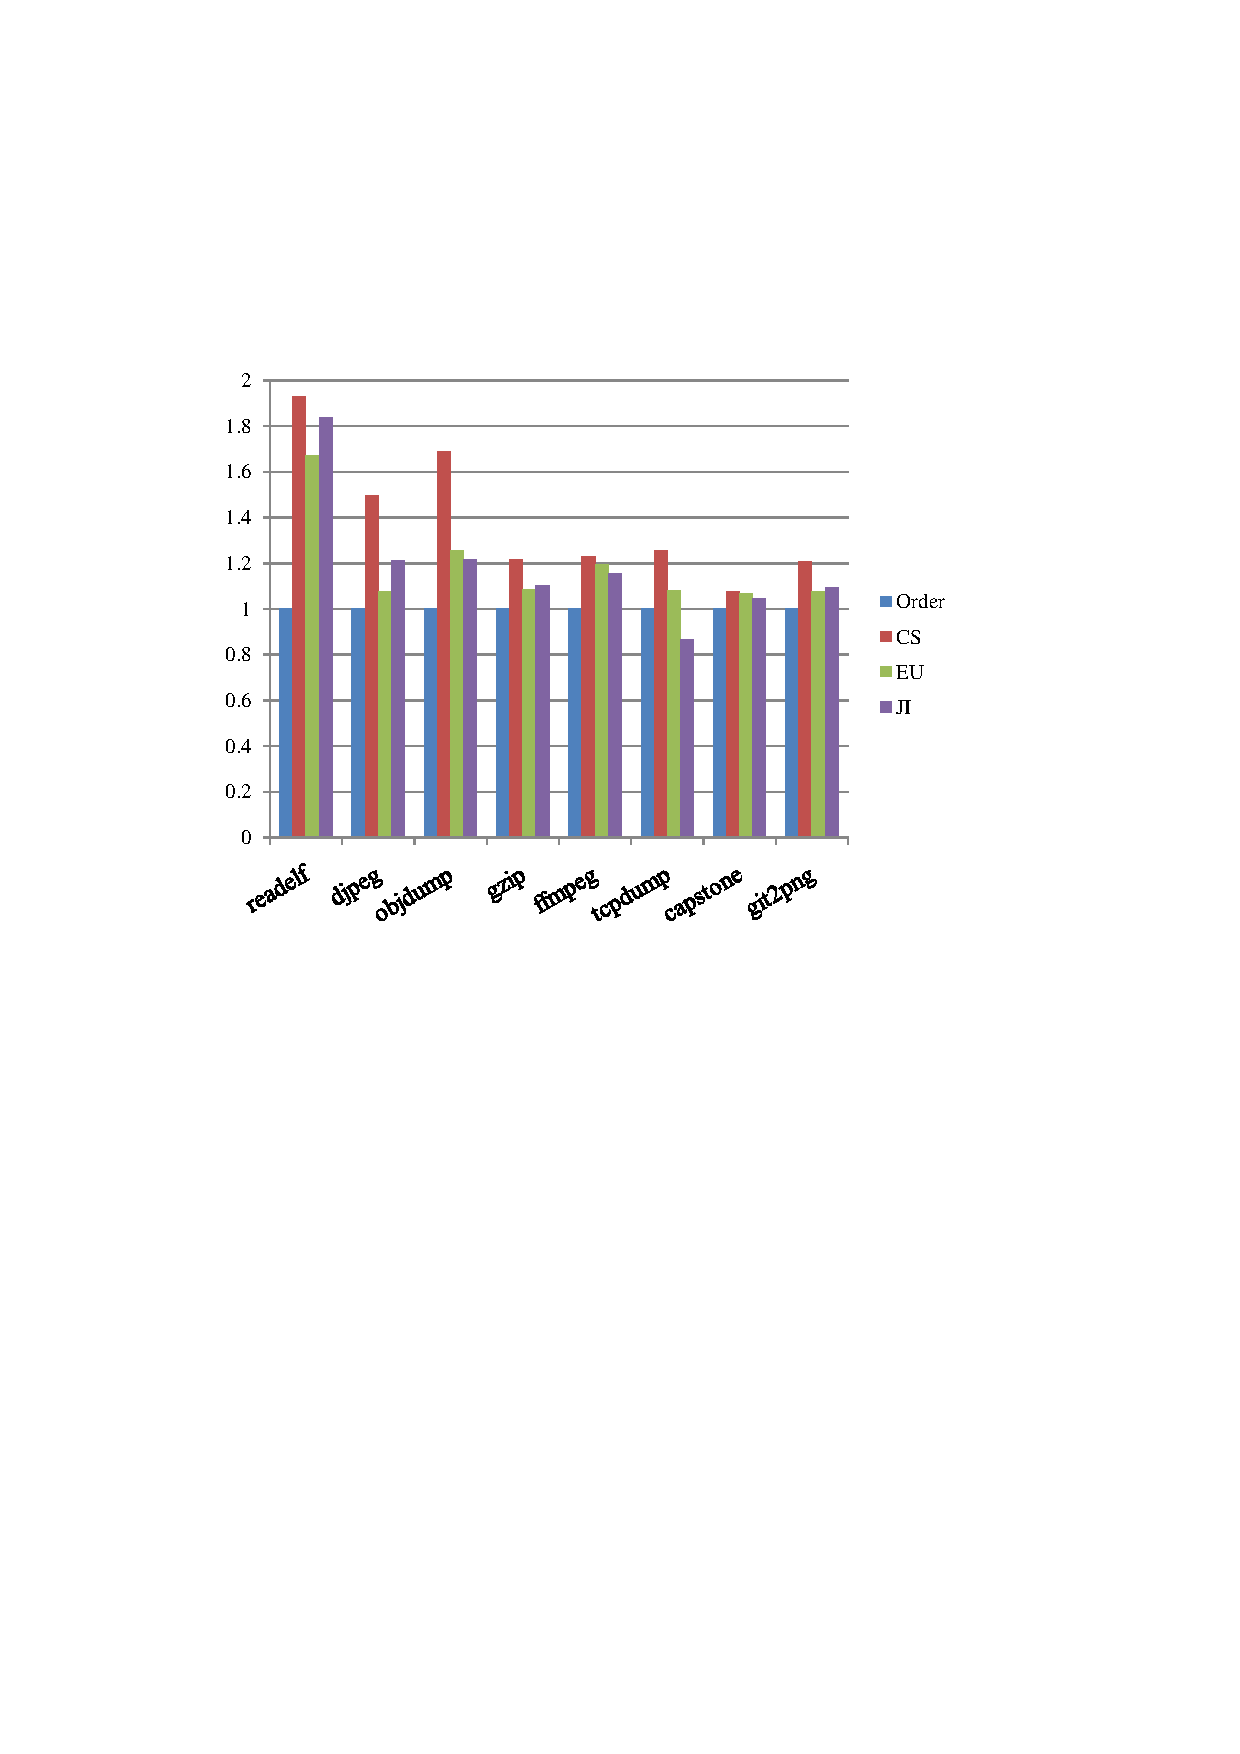
\includegraphics[width=0.8\textwidth]{figures/path-discovery.pdf} 
\caption{Path Discovery for different search strategies.}\label{path-discovery}
\end{figure}
\begin{figure}
\centering
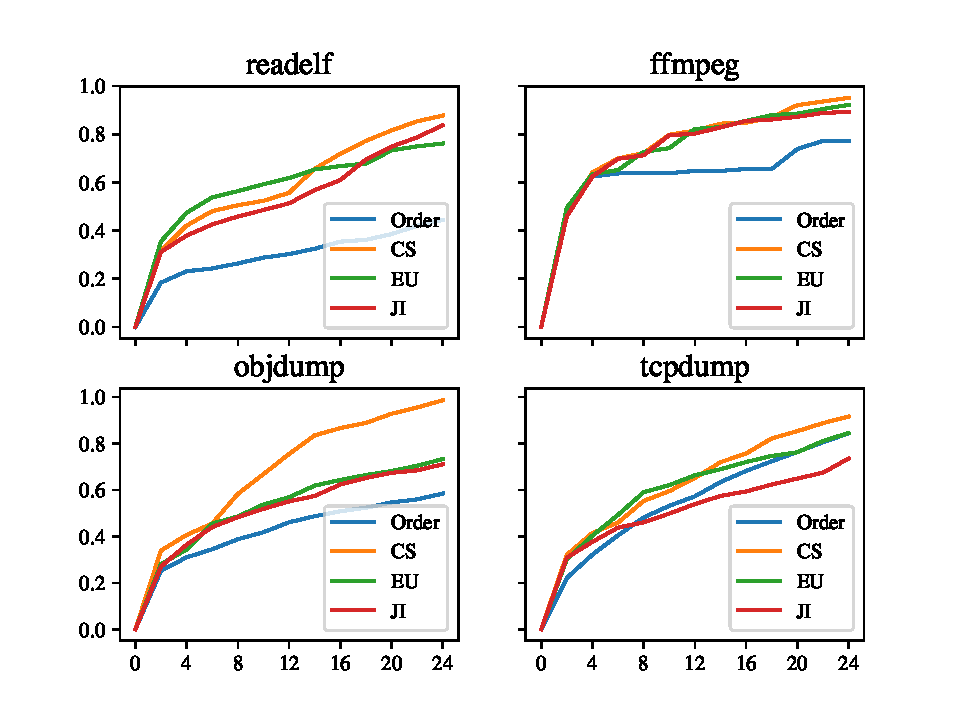
\includegraphics[width=0.8\textwidth]{figures/path-time-detail.pdf} 
\caption{Path Discovery for different search strategies within 24 hours.}\label{path-detail}
\end{figure}
\subsection{Bug Finding}
In this section, we evaluated our method with two different benchmarks. And we also compared the results of the other off-the-shelf vulnerability discovery tools, which are LibFuzzer, AFL, KLEE, S2E, and Driller.

The first benchmark is a demo program which is named as \emph{CommonMB}. The second benchmark is \emph{LAVA}, which is released in 2016 to test different vulnerability discovery tools. We will introduce the two benchmarks and the testing results in detail in the following.


\subsubsection{CommonMB}~\par
\vskip0.5mm
\noindent The \emph{CommonMB} benchmark is a demo program which contains 9 different memory error bugs. These bugs can be triggered only when feeding the program with specifically crafted input. There are four different kinds of functions in this benchmark, i.e. 2 compare-style functions, 3 math-style functions, 2 checksum-style functions and 2 logic-style functions. The compare functions contains bugs that can only be triggered when the values of specific parts of the input equal to specific constant immediate numbers; the bugs in math functions can be triggered when the results of math operation on some specific parts of the input equal to specific constant immediate numbers; the checksum related bugs can only be triggered when the input data successfully goes through the checksum checking points; and the logic bugs utilize two simple logical games (maze and semi-sudoku) as the constraints for triggering the bugs, which means the bugs can only be triggered when the testing engine successfully solves the games.

Table~\ref{CommonMB-results} shows the overall results of different vulnerability discovery tools as well as our prototype with same test environment (10 cores and 24 hours). 

Table~\ref{Prototype-result-CommonMB} shows the bug finding evaluation results of our prototype on CommonMB benchmark. The first column lists the number of cores for the concolic execution engine, and we have tested from one core to 10 cores and collected the discovery time for each bug. 

\begin{table}
  \caption{\label{CommonMB-results}Evaluation results on \textit{CommonMB}}
  \centering
	\begin{tabular}{p{2cm}<{\centering} p{2cm}<{\centering} p{3cm}<{\centering} p{1.5cm}<{\centering}}
		\toprule
		Tool                     & target   & method                  & Triggered Bugs\# \\ \midrule
		AFL                      & Binary   & Fuzz                    & 3             \\
		LibFuzzer                & Source   & Fuzz                    & 4             \\
		KLEE                     & Source   & Symbex                  & 3             \\
		S2E                      & Binary   & Symbex                  & 7             \\
		Driller                  & Binary   & Symbex + Fuzz           & 5             \\
		Prototype                & Binary   & Symbex + Fuzz           & 8             \\ \bottomrule
	\end{tabular}
\end{table}

\begin{table}
  \caption{\label{CommonMB-results-detail}Evaluation results on \textit{CommonMB} in detail}
  \centering
	\begin{tabular}{p{2cm}<{\centering} p{1cm}<{\centering} p{1cm}<{\centering} | p{1cm}<{\centering}
	p{1cm}<{\centering} p{1.2cm}<{\centering} | p{1cm}<{\centering} p{1cm}<{\centering} | p{1cm}<{\centering} p{1cm}<{\centering}}
		\toprule
	& \multicolumn{2}{c}{CMP}  & \multicolumn{3}{c}{MATH} & \multicolumn{2}{c}{CHECKSUM} & 	\multicolumn{2}{c}{LOGIC} \\ 
	    Tool & cmp16 & cmp32 & add16 & add32 & complex & crc16 & crc32 & maze & sudoku \\
		\midrule
		AFL 		& Y & Y & Y & N & N & N & N & N & N \\
		LibFuzzer	& Y & Y & Y & Y & N & N & N & N & N \\
		KLEE		& Y & Y & Y & N & N & N & N & N & N \\
		S2E			& Y & Y & Y & Y & Y & Y & Y & N & N \\
		Driller		& Y & Y & Y & Y & Y & N & N & N & N \\
		Prototype	& Y & Y & Y & Y & Y & Y & Y & Y & N \\
	 \bottomrule
	\end{tabular}
\end{table}
\begin{table}
\centering
  \caption{\label{Prototype-result-CommonMB}Trigger time for each bug in \textit{CommonMB}  of our prototype (in \textit{second}).}
 	\begin{tabular}{p{0.5cm}<{\centering} p{1cm}<{\centering} p{1cm}<{\centering} p{1cm}<{\centering}	p{1cm}<{\centering} p{1.5cm}<{\centering}  p{1cm}<{\centering} p{1cm}<{\centering}  p{1.5cm}<{\centering} p{1.5cm}<{\centering}}
		\toprule
	    Core & cmp16 & cmp32 & add16 & add32 & complex & crc16 & crc32 & maze & sudoku \\
		\midrule
		1 	& 4.69 & 6.32 & 4.68 & 5.72 & $>1$ hour & 5.88 & 185.66 & $>1$ hour & $>1$ hour \\
		2	& 0.02 & 2.44 & 4.31 & 0.74 & $>1$ hour & 5.14 & 2.51   & $>1$ hour & $>1$ hour \\
		4	& 0.02 & 0.24 & 4.06 & 0.32 & $>1$ hour & 4.59 & 1.50   & $>1$ hour & $>1$ hour \\
		6	& 0.02 & 0.21 & 4.16 & 0.14 & 0.48 	    & 4.67 & 2.80   & $>1$ hour & $>1$ hour \\
		8	& 0.05 & 0.21 & 4.09 & 0.15 & 1.57      & 4.58 & 1.52   & $>1$ hour & $>1$ hour \\
		10	& 0.02 & 0.20 & 4.08 & 0.30 & 1.54      & 4.57 & 1.53   & 10.86     & $>1$ hour \\
	 \bottomrule
	\end{tabular}
\end{table}



\subsubsection{LAVA}~\par
\vskip0.5mm
\noindent In 2016, Dolan-Gavitt et.al. developed a technique, namely LAVA, to automatically inject secure-related bugs into some Linux utilities for evaluating the bug-finding tools. These bugs are all hard-to-reach memory errors. In the paper of LAVA, the authors describe their results on the evaluation of coverage based fuzz testing, an SAT-based approach on the benchmark. The LAVA benchmark has two corpus sets, i.e. \textit{LAVA-1} and \textit{LAVA-M}.

\textit{LAVA-1} injected 69 different bugs into the \texttt{file} program in Linux CoreUtils. There are two types of buffer overflow vulnerabilities were injected, one is \emph{Range} and the other one is \emph{Knob-and-trigger (KT)}. The Range style bugs trigger if the magic value is in some range and also check the value to determine how much to overflow. And in the KT bug, two bytes in the input are checked against a magic value to determine if the overflow will happen and another two bytes determine how much to overflow. Both the two types of bugs were designed to mirror real bug patterns which can be used to evaluate the ability of bug-finding tools. Compared \textit{LAVA-1}, which injected only one bug in the program, \textit{LAVA-M} injected more than one bug into four different programs in CoreUtils that took file input: \texttt{base64}, \texttt{md5sum}, \texttt{uniq}, and \texttt{who}, so \textit{LAVA-M} is a better benchmark to evaluate the vulnerability discovery tools that are designed to work for a long time on programs that may contain multiple bugs.

\begin{table}
  \caption{\label{LAVA-1}Evaluation results on \textit{LAVA-1}.}
  \centering
	\begin{tabular}{p{2cm}<{\centering} p{1.5cm}<{\centering} p{1.6cm}<{\centering}  p{1.6cm}<{\centering}	p{1.5cm}<{\centering} p{1.5cm}<{\centering}  p{1.5cm}<{\centering} }
		\toprule
	    Tool & $2^0$ & $2^7$  & $2^{14}$ & $2^{21}$ & $2^{28}$ & KT \\
	         & (12 bugs) & (10 bugs) & (11 bugs) & (14 bugs) & (12 bugs) & (10 bugs) \\
		\midrule
		FUZZER 		& 0 (0\%)   & 0 (0\%)    & 1 (9\%)    & 11 (79\%) & 9 (75\%)  & 2 20\%) \\
		SES	        & 1 (8\%)   & 0 (0\%)    & 1 (9\%)    & 3 (21\%)  & 0 (0\%)   & 1 (10\%) \\
		AFL		    & 0 (0\%)   & 0 (0\%)    & 2 (18\%)   & 10 (71\%) & 9 (75\%)  & 1 (10\%) \\
		S2E			& 3 (25\%)  & 2 (20\%)   & 3 (27\%)   & 4 (27\%)  & 3 (25\%)  & 2 (20\%) \\
		Driller		& 1 (8\%)   & 2 (20\%)   & 2 (18\%)   & 12 (86\%) & 10 (73\%) &  (10\%) \\
		Prototype	& 10 (83\%) & 10 (100\%) & 11 (100\%) & 13 (93\%) & 11 (92\%) & 7 (70\%) \\
	 \bottomrule
	\end{tabular}
\end{table}

Table~\ref{LAVA-1} summarized the results of bug finding evaluation on \textit{LAVA-1} from LAVA paper as well as some popular off-the-shelf tools (AFL/S2E/Driller). The maximum testing time for each bug was five hours. From this table, we can see that the \textbf{FUZZER} and \textbf{SES} mentioned in the paper only found 23 bugs and 6 bugs respectively in total. AFL found fewer paths than S2E in the small ranges ($2^0$, $2^7$ and $2^{14}$) but it outperformed S2E in larger ranges. Driller leverages the advantages of both fuzz testing and symbolic execution and the results show that it can find more paths than using them separately (28 bugs were discovered in total).

While our prototype discovered 62 bugs which was much more than the FUZZER and the SES tools separately. Particularly, we triggered all the bugs in $2^7$ and $2^{14}$ ranges. And also found most of the KT bugs (70\%) which cannot be touched effectively by the FUZZER and SES tools. Meanwhile, because of the two improvements (i.e. \textit{SLB} and \textit{LSP}), our prototype can also trigger more bugs than Driller.

Table~\ref{LAVA-M} describes the evaluation results on LAVA-M of the FUZZER and SES which are mentioned in the LAVA paper. We also listed the results of VUzzer and our prototype. 

\begin{table}
  \caption{\label{LAVA-M}Evaluation results on \textit{LAVA-M}.}
  \centering
	\begin{tabular}{p{2cm}<{\centering} p{1.5cm}<{\centering} p{1.5cm}<{\centering}  p{1.5cm}<{\centering} p{1.8cm}<{\centering}  p{1.5cm}<{\centering} }
		\toprule
	    Tool & \texttt{base64} & \texttt{md5sum} & \texttt{uniq} & \texttt{who} & Total  \\
	         & (44 bugs) & (57 bugs) & (28 bugs) & (2136 bugs) &  \\
		\midrule
		FUZZER 		& 7  & 2  & 7    & 0   & 16  \\
		SES	        & 9  & 0  & 0    & 18  & 27  \\
		VUzzer		& 17 & 1* & 27   & 50  & 95 \\
		Prototype	& 37 & 29 & 28   & 203 & 297 \\
	 \bottomrule
	\end{tabular}
\end{table}

As mentioned in the paper of LAVA, SES cannot find any bugs in \texttt{uniq} and \texttt{md5sum}. And the reasons are the control flow is too unconstrained in \texttt{uniq} and SES failed to execute any code past the first instance of the hash function. Because our symbolic execution is driven by a concrete seed input, so these two problems will be eased to a large extent which led to finding more bugs. Particularly, for program \texttt{md5sum}, VUzzer can only trigger one bug because it fails to get through the first crash to parse more of any input, whereas our prototype successfully triggered 29 bugs in \texttt{md5sum}.